
\documentclass{beamer}
\usetheme{Montpellier} 
\usecolortheme{dolphin} 
\usepackage{parskip}
\setlength{\parskip}{\smallskipamount} 
\usepackage{array}
\usepackage{fancybox}
\usepackage{mathrsfs}

\usepackage{enumerate}
\usepackage{amsmath,amsthm,amssymb}
\usepackage{mathrsfs} % to use mathscr fonts

\usepackage{pstricks}
\usepackage{pst-solides3d}
\usepackage{pstricks-add}
\usepackage{graphicx}
\usepackage{pst-tree}
\usepackage{pst-poly}
\usepackage{calc,ifthen}
\usepackage{float}\usepackage{multicol}
\usepackage{multirow}
\usepackage{array}
\usepackage{longtable}
\usepackage{tikz}
\usepackage{tkz-berge}
\usepackage{fancyhdr}
\usepackage{algorithmicx,algpseudocode}
\usepackage{changepage}
\usepackage{color}
\usepackage{listings}
\usepackage{fancyvrb}

\title{Extremal Cayley Graphs}
\author{Jordan Blocher, Christopher Linden,  Samantha Hampton}
\date{\today}
\institute[2008]{REU - Texas State}

 \def\ddd{\displaystyle}
 \def\R{\mbox{$\mathbb R$}}
 \def\Q{\mbox{$\mathbb Q$}}
 \def\Z{\mbox{$\mathbb Z$}}
 \def\N{\mbox{$\mathbb N$}}
 \def\C{\mbox{$\mathbb C$}}


\def\Sym{\operatorname{Sym}}
\def\lcm{\operatorname{lcm}}
\def\adj{\operatorname{adj}}
\def\inc{\operatorname{inc}}
\def\Cay{\operatorname{Cay}}
\def\Geom{\operatorname{\cal G}}
\def\diam{\operatorname{diam}}
\def\rank{\operatorname{rank}}
\def\n{\\ \vspace{1.7mm}}

\lstset{ %
language=C++,                % choose the language of the code
basicstyle=\footnotesize,       % the size of the fonts that are used for the code
numbers=none,                   % where to put the line-numbers
numberstyle=\footnotesize,      % the size of the fonts that are used for the line-numbers
stepnumber=1,                   % the step between two line-numbers. If it is 1 each line will be numbered
numbersep=5pt,                  % how far the line-numbers are from the code
backgroundcolor=\color{white},  % choose the background color. You must add \usepackage{color}
showspaces=false,               % show spaces adding particular underscores
showstringspaces=false,         % underline spaces within strings
showtabs=false,                 % show tabs within strings adding particular underscores
frame=none,           % adds a frame around the code
tabsize=2,          % sets default tabsize to 2 spaces
captionpos=b,           % sets the caption-position to bottom
breaklines=true,        % sets automatic line breaking
breakatwhitespace=false,    % sets if automatic breaks should only happen at whitespace
escapeinside={\%*}          % if you want to add a comment within your code
}



\begin{document}


\frame{\titlepage}
\frame{
	\frametitle{\underline{Introduction to Cayley Graphs}}
\begin{center}
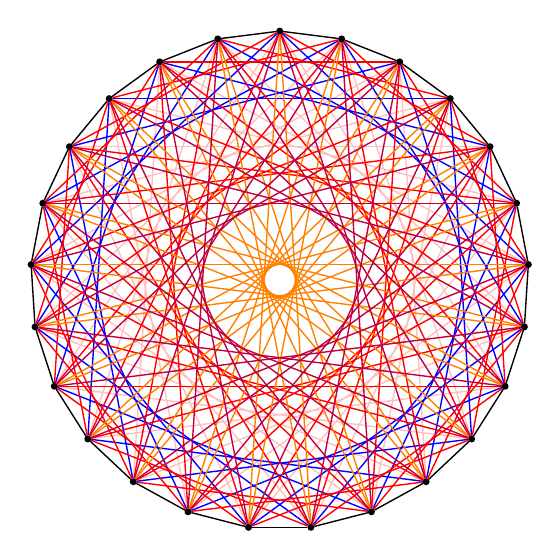
\begin{tikzpicture}[scale=.6]


\GraphInit[vstyle=Simple]
\tikzset{VertexStyle/.append style = {minimum size =2pt, inner sep = 0pt}}


\Vertex[x=187.5pt,y=337.5pt]{0};
\Vertex[x=224.80348307472823pt,y=332.7874741692947pt]{1};
\Vertex[x=259.7630511152573pt,y=318.94600200657953pt]{2};
\Vertex[x=290.1820658893033pt,y=296.8452941132117pt]{3};
\Vertex[x=314.14918882530225pt,y=267.87401924684946pt]{4};
\Vertex[x=330.15847744427305pt,y=233.85254915624213pt]{5};
\Vertex[x=337.2040092642407pt,y=196.91857792939703pt]{6};
\Vertex[x=334.8430876093033pt,y=159.3928028121413pt]{7};
\Vertex[x=323.22405786990294pt,y=123.63310626523908pt]{8};
\Vertex[x=303.0769864163684pt,y=91.88640153769651pt]{9};
\Vertex[x=275.667787843871pt,y=66.14745084375791pt]{10};
\Vertex[x=242.71868290270174pt,y=48.0335271167623pt]{11};
\Vertex[x=206.2999850346457pt,y=38.682794802828326pt]{12};
\Vertex[x=168.70001496535434pt,y=38.682794802828326pt]{13};
\Vertex[x=132.2813170972983pt,y=48.03352711676226pt]{14};
\Vertex[x=99.3322121561291pt,y=66.14745084375782pt]{15};
\Vertex[x=71.92301358363159pt,y=91.88640153769656pt]{16};
\Vertex[x=51.77594213009703pt,y=123.63310626523916pt]{17};
\Vertex[x=40.1569123906967pt,y=159.3928028121413pt]{18};
\Vertex[x=37.795990735759275pt,y=196.91857792939695pt]{19};
\Vertex[x=44.841522555726954pt,y=233.8525491562421pt]{20};
\Vertex[x=60.85081117469775pt,y=267.8740192468495pt]{21};
\Vertex[x=84.81793411069665pt,y=296.8452941132117pt]{22};
\Vertex[x=115.23694888474257pt,y=318.9460020065795pt]{23};
\Vertex[x=150.1965169252717pt,y=332.7874741692946pt]{24};

\SetUpEdge[lw         = .5pt,
            color      = black,
            labelcolor = black]

\Edge(24)(0)
\Edge(0)(1)
\Edge(1)(2)
\Edge(2)(3)
\Edge(3)(4)
\Edge(4)(5)
\Edge(5)(6)
\Edge(6)(7)
\Edge(7)(8)
\Edge(8)(9)
\Edge(9)(10)
\Edge(10)(11)
\Edge(11)(12)
\Edge(12)(13)
\Edge(13)(14)
\Edge(14)(15)
\Edge(15)(16)
\Edge(16)(17)
\Edge(17)(18)
\Edge(18)(19)
\Edge(19)(20)
\Edge(20)(21)
\Edge(21)(22)
\Edge(22)(23)
\Edge(23)(24)

\SetUpEdge[lw         = .5pt,
            color      =pink,
            labelcolor = black]

\Edge(0)(8)
\Edge(2)(10)
\Edge(4)(12)
\Edge(6)(14)
\Edge(8)(16)
\Edge(10)(18)
\Edge(12)(20)
\Edge(14)(22)
\Edge(16)(24)
\Edge(18)(1)
\Edge(20)(3)
\Edge(22)(5)
\Edge(24)(7)
\Edge(1)(9)
\Edge(3)(11)
\Edge(5)(13)
\Edge(7)(15)
\Edge(9)(17)
\Edge(11)(19)
\Edge(13)(21)
\Edge(15)(23)
\Edge(17)(0)
\Edge(19)(2)
\Edge(21)(4)
\Edge(23)(6)

\SetUpEdge[lw         = .5pt,
            color      =blue,
            labelcolor = black]

\Edge(0)(6)
\Edge(6)(12)
\Edge(12)(18)
\Edge(18)(24)
\Edge(24)(5)
\Edge(5)(11)
\Edge(11)(17)
\Edge(17)(23)
\Edge(23)(4)
\Edge(4)(10)
\Edge(10)(16)
\Edge(16)(22)
\Edge(22)(3)
\Edge(3)(9)
\Edge(9)(15)
\Edge(15)(21)
\Edge(21)(2)
\Edge(2)(8)
\Edge(8)(14)
\Edge(14)(20)
\Edge(20)(1)
\Edge(1)(7)
\Edge(7)(13)
\Edge(13)(19)
\Edge(19)(0)

\SetUpEdge[lw         = .5pt,
            color      =red,
            labelcolor = black]

\Edge(0)(4)
\Edge(4)(8)
\Edge(8)(12)
\Edge(12)(16)
\Edge(16)(20)
\Edge(20)(24)
\Edge(24)(3)
\Edge(3)(7)
\Edge(7)(11)
\Edge(11)(15)
\Edge(15)(19)
\Edge(19)(23)
\Edge(23)(2)
\Edge(2)(6)
\Edge(6)(10)
\Edge(10)(14)
\Edge(14)(18)
\Edge(18)(22)
\Edge(22)(1)
\Edge(1)(5)
\Edge(5)(9)
\Edge(9)(13)
\Edge(13)(17)
\Edge(17)(21)
\Edge(21)(0)
\Edge(0)(9)
\Edge(9)(18)
\Edge(18)(2)
\Edge(2)(11)
\Edge(11)(20)
\Edge(20)(4)
\Edge(4)(13)
\Edge(13)(22)
\Edge(22)(6)
\Edge(6)(15)
\Edge(15)(24)
\Edge(24)(8)
\Edge(8)(17)
\Edge(17)(1)
\Edge(1)(10)
\Edge(10)(19)
\Edge(19)(3)
\Edge(3)(12)
\Edge(12)(21)
\Edge(21)(5)
\Edge(5)(14)
\Edge(14)(23)
\Edge(23)(7)
\Edge(7)(16)
\Edge(16)(0)


\SetUpEdge[lw         = .5pt,
            color      = orange,
            labelcolor = black]

\Edge(24)(12)
\Edge(0)(13)
\Edge(1)(14)
\Edge(2)(15)
\Edge(3)(16)
\Edge(4)(17)
\Edge(5)(18)
\Edge(6)(19)
\Edge(7)(20)
\Edge(8)(21)
\Edge(9)(22)
\Edge(10)(23)
\Edge(11)(24)
\Edge(12)(0)
\Edge(13)(1)
\Edge(14)(2)
\Edge(15)(3)
\Edge(16)(4)
\Edge(17)(5)
\Edge(18)(6)
\Edge(19)(7)
\Edge(20)(8)
\Edge(21)(9)
\Edge(22)(10)
\Edge(23)(11)


\SetUpEdge[lw         = .5pt,
            color      = purple,
            labelcolor = black]

\Edge(24)(9)
\Edge(0)(10)
\Edge(1)(11)
\Edge(2)(12)
\Edge(3)(13)
\Edge(4)(14)
\Edge(5)(15)
\Edge(6)(16)
\Edge(7)(17)
\Edge(8)(18)
\Edge(9)(19)
\Edge(10)(20)
\Edge(11)(21)
\Edge(12)(22)
\Edge(13)(23)
\Edge(14)(24)
\Edge(15)(0)
\Edge(16)(1)
\Edge(17)(2)
\Edge(18)(3)
\Edge(19)(4)
\Edge(20)(5)
\Edge(21)(6)
\Edge(22)(7)
\Edge(23)(8)

\end{tikzpicture}
\end{center}

\begin{itemize}
		\item<1->
\begin{center}
Cay($\mathbb{Z}_{25}$, \{$\pm$1,$\pm$4,$\pm$6,$\pm$8, $\pm10$, $\pm$13\})     
\end{center}
                 
\end{itemize}
}

\frame {
	\frametitle{\underline{Introduction to Cayley Graphs}}
	\only<1>{
	\begin{itemize}
                  \item<1-> Definition:  Let $\Gamma$ be a finite group with a subset $\mathscr{A}$. The {\emph{Cayley digraph}}, denoted $\Cay(\Gamma,\mathscr{A})$, is a digraph with vertex set $\Gamma$, such that (x,y) is a directed edge if and only if $yx^{-1} \in \mathscr{A}$.

		\item<1->\emph{Cayley digraphs} are vertex transitive.
		\item<1->The Cayley digraph of a finit cyclic group is called a circulant graph.  Our project focuses on circulant graphs.

	\end{itemize}
}
}

\frame {
	\frametitle{\underline{Introduction to Cayley Graphs}}
	\only<1>{
	\begin{itemize}
                  \item<1-> For a positive integer $d$ and a subset of integers $\mathscr{A}$ we define :
\begin{align*}
m(d,\mathscr{A}) &=\max\{m | \diam(\Cay(\mathbb{Z}_m,\mathscr{A})) \leq d\} \text{,} \\
\end{align*}
\item<1-> For positive integers $d$ and $k$ we define
\begin{align*}
m(d,k) &= \max_{|A| = k}\{m(d,A)  \}.
\end{align*}
	\end{itemize}
}
}


\frame{
	\frametitle{\underline{Introduction to Cayley Graphs}}
	\only<1>{
	\begin{itemize}
                  \item<1-> Current known values include:
\begin{align*}
m(1,k) &= k+1,
\\
\textcolor{blue}{m(2,k)} &\geq \textcolor{blue}{\frac{37}{121}k^2 + O(k)},
\\
m(d,1) &= d+1\text{, and}
\\
m(d,2) &= \left\lfloor \frac{d(d+4)}{3} \right\rfloor+1 \text{ for all } d\geq2.
\end{align*}

	\end{itemize}
}
}

\frame{
	\frametitle{\underline{Finding lower bounds on m(d,k)}}
	\only<1>{
	\begin{itemize}
                  \item<1-> For a (small) fixed k, we can give a set $\mathscr{A}$ the $k$ elements of which are written in terms of $d$.  If we can prove that $d\mathscr{A}$ always contains $\Z_m$ for some $m$, also a function of $d$, then we have a lower bound for $m(d,k)$.
                  \item<1-> For example, the set $\mathscr{A} = \{1, 3d -8\lfloor{\frac{d}{4}}\rfloor +5, \lfloor{\frac{d}{4}}\rfloor(3d -8\lfloor{\frac{d}{4}}\rfloor +5) +d - 3\lfloor{\frac{d}{4}}\rfloor \}$ generates $m = \frac{d^3}{16} + \frac{3d^2}{8} + O(d)$, so $m(d,3) \ge \frac{d^3}{16} + O(d^2)$.

	\end{itemize}
}
}

\frame{
	\frametitle{\underline{Finding lower bounds on m(d,k)}}
	\only<1>{
	\begin{itemize}
                  \item<1-> If the sets $\mathscr{A}$ and values $m$ are of a particular form, it is possible to have a computer check whether or not  $d\mathscr{A} \supset \Z_m$. 
                  \item<1-> We can then (in theory) have the computer loop though all possible generating sets and moduli of this particular form to search for new lower bounds.
                  \item<1->In practice, this may be computationally infeasible.

	\end{itemize}
}
}

\frame{
	\frametitle{\underline{The Algorithm}}
	\only<1>{
    \begin{itemize}
        \item<1->Designed iterate through permutations of the generating set and possible coverings, giving as an output the maximal generating set as well as the optimal polynomial bound. 
        \item<1->The algorithm takes advantage of the fact that there exists a one-to-one correspondance between representations of the residual classes of $\Z_m$ and the set of integers $[0, m-1]$.
    \end{itemize}
}}

\frame{
	\frametitle{\underline{Polynomial Construction}}
	\only<1>{
    \begin{itemize}
    \item<1->Let $d$ be the diameter for $\Cay(m, \mathscr{A})$.
    \item<1->Our lower bound on $m(d, k)$ will be defined as a polynomial in terms of $\lambda$. 
    \end{itemize}
\n
$\lambda$ is a large number determined by $d$. The parameter $\lambda$ will not appear in the code, but it enables us to compute a lower bound as a function of $d$.
\n
Given $d$ define \emph{\bf{$d_{1}$ fixed}} to be $\frac{d}{\lambda}$. This will be the $d$ referred to in the algorithm.\n
}}

\frame{
	\frametitle{\underline{Data Structures}}
	\only<1>{
\noindent
The purpose of the data structures is to provide containers for the following:\n
    \begin{itemize}
    \item<1->Define $\mathscr{A}$ to be a \emph{set of generators}, $\mathscr{A} = (a_{i})$ such that $ a_{i} = \alpha_{i+1}a_{i+1}\lambda,  \forall i \in [0, k-1] $, where $a_i$ a sequence of nonnegative coefficients, and $\vert \mathscr{A} \vert = k$.\n
    \item<1->Define a \emph{set of non-negative coefficients} $c_1, c_2, .. , c_k$ such that $c_{i+1} < \alpha_{i} \lambda$.\n
    \item<1->Lastly, define a \emph{second set of non-negative coefficients} $x_1, x_2, .., x_{k}$ such that $x_{i+1} < d - \sum_{0}^{i}x_i$.
    \end{itemize}
\n \noindent
Assume that the set of generator combinations is defined as an upper-triangular two-dimensional array of unordered coefficients represented by tuples, the sequences of coefficients are defined as ordered lists of tuples.
}}

\frame{
	\frametitle{\underline{Polynomial Representation}}
	\only<1>{
 Our representative polynomial can now be defined.
\begin{align*}
m(d, k) &= a_{1}c_{1} + a_{2}c_{2} \cdots + a_{k}c_{k} 
\\
&= (\Pi_{1}^{k}\alpha_{i})c_{1}\lambda^k + (\Pi_{2}^{k}\alpha_{i})c_{2}\lambda^{k-1} \cdots (\alpha_{k})c_{k}\lambda
\end{align*}
\noindent
For all constructed polynomials $x = x_1a_{1} + x_2a_{2} + .. + x_{k}a_{k}$, we define a representative $x' \in [1, m-1]$ to which we will map all congruent polynomials, forming our residue class $\bar{x}$ of regular polynomials.\n
}}

\frame{
	\frametitle{\underline{Polynomial Representation}}
	\only<1>{
    \begin{itemize}
    \item<1->The constructed polynomial $x$ is defined to be \textbf{regular} if $x \in [0, m-1]$.
    \item<1->$ \{ (x_1, x_2, ... , x_k) \vert x_{1} \leq c_1, x_{2} \leq c_2, .. , x_{k} \leq c_k$, and $\sum_{i} x_i \leq d_{1} \}$ define polynomials $x$ that are considered to be \textbf{minimal}.\n
    \end{itemize}
\n
We will use regular polynomials to determine whether or not $d \mathscr{A} = \Z_m$ by only considering a single covering of $\Z_m$.\n
\noindent
Note that a regular polynomial need not be minimal.\n
\noindent
We check for regularity by comparing the coefficients $(x_1, x_2, .. , x_{k})$ and $(c_1, c_2, .. , c_k)$ from their respective polynomials.\n
}}

\frame{
	\frametitle{\underline{Polynomial Representation}}
	\only<1>{
    \begin{itemize}
    \item<1->$\forall x \in d \mathscr{A}$ if $x \notin [0, m-1]$, we can identify $x$ with point $x' = (x'_1, x'_2, .. , x'_k) \in [0, m-1]$ congruent to $x$ $(mod$ $m)$.  Then if every point $n \in \Z_m$ is either equal to some $x$ or $x'$, then $d \mathscr{A} \cong \Z_m$.\n
    \end{itemize}
\noindent
The number of times that the representative set cycles $\Z_m$ as well as the number of times that a generator needs to be "borrowed" into the next lowest-order term is saved to use to create the intervals bounding the representative coefficients in the mathematical proof.
}}

\frame{
	\frametitle{\underline{Parallelization}}
	\only<1>{
The looping nature of the program makes it a natural candidate for optimization using parallel processing techniques. The largest dataset that is iterated over is the M-Coefficients, and can be a "bottleneck" in the program. Parallelization solves this problem by allowing a number of nodes that compute extremely large datasets to compute for an extended time or even without completion. These larger computations will not interfere with nodes that are computing bounds based on subsequent generating sets. The effect of the multiple processes is that we are able to check a larger set of generators, in fact checking up to the current trivial lower bound of $\frac{d^k}{k!}$.
}}

\frame{
	\frametitle{\underline{Complexity}}
	\only<1>{
The generation of the polynomial bound is again a nested loop structure which checks each possible representative for each possible combination for each generating set that can be created where each generator is the largest possible multiple it can take for its position up to the trivial upper bound. 
    \begin{itemize}
    \item<1->We can describe the complexity of this main program as $\mathcal{O}(d^k) \cdot \Theta(d^k) \cdot \mathcal{O}(d^k) = \mathcal{O}(d^{k^3})$.
    \end{itemize}
    As we found, the size of the coefficient set for the polynomial bound depends largely on the specific generating set being examined, significantly affecting the complexity of the inner loops (or coefficient loops).
}}


\frame{
    \frametitle{\underline{Future Work}}
    \only<1>{
        Upon completion, the results from the current implementation of the algorithm in C++ did not give an improvement to current lower bound for $k = 3, 4, 5, 6$. It was decided that improvements to the accuracy of the polynomial representation were needed in order to improve the result. Towards this effort, we extend each generator to include lower-order polynomial terms.

        We now define $\mathscr{A}$ to be a \emph{set of generators}, $\mathscr{A} = \{a_{i}\}$ such that $a_{i+1} = \sum_{i}^{k}\alpha_{ij}a_{j},  \forall i \in [1, k-1] $, with $\{a_i\}$ a sequence of polynomial representations, and $\vert \mathscr{A} \vert = k$.\n
}}

\frame{
    \frametitle{\underline{Construction of the Generating Set for $k=6$}}
    \only<1>{

\lstinline{typedef Tuple<int, k> T;}

\lstinline{// Construction of Generators}

\lstinline{A[0] = (N, I1, J1, K1, L1, 0);}

\lstinline{A[1] = (0, I2, J2, K2, L2, 0);}

\lstinline{A[2] = (0, 0, J3, K3, L3, 0);}

\lstinline{A[3] = (0, 0, 0, K4, L4, 0);}

\lstinline{A[4] = (0, 0, 0, 0, L5, 0);}

\lstinline{A[5] = (0, 0, 0, 0, 0, 1);}

}}


\frame{
    \frametitle{Polynomial Data Structure}
    \only<1>{
        
    The basic polynomial data structure uses a 2D upper-triangular array to store the generating set.

\lstinline{class Polynomial}
\{

\lstinline{Tuple A[k];  // container for Generators}

\lstinline{Tuple Y;  // container for M-Coefficients or X-Coefficients}

\lstinline{int subtractions[k];}

\}

In the case where Polynomial \lstinline{P.Y} is a container for the M or X-Coefficients, the class instance is a representation of the polynomial $x$ or $X'$.
\lstinline{P.Y[0]} will refer to the largest polynomial coefficient. \lstinline{P.A[i][0]} will refer to the largest corresponding generator where $i = 1, 2, \cdots, k$.
}}

\frame{
	\frametitle{\underline{Analysis}}
	\only<1>{
 The complexity of the loop constructing the generators has increased to $\mathcal{O}(d^{k^2})$, increasing the complexity of the complete algorithm is $\mathcal{O}(d^{k^4})$.
                  
}}


\frame{
	\frametitle{\underline{The General Case}}
	\only<1>{
	\begin{itemize}
                  \item<1-> One of the reasons we are interested in lower bounds on $m(d,k)$ for specific values of $k$ is because we can use them to obtain a lower bound for arbitrary $k$ as $d \to \infty$.
                  \item<1-> We use the inequality
\[
	m(d_1+d_2,k_1+k_2) \ge m(d_1,k_1)m(d_2,k_2)
\]
to establish these general case bounds.
				\item<1-> We can also use it to find bounds for arbitrary $d$ as $k \to \infty$.                
	\end{itemize}
}
}

\frame{
	\frametitle{\underline{The General Case: example proof}}
	\only<1>{
	\begin{itemize}
                  \item<1-> Using our $m(2,k)$ result, we prove a lower bound on $m(d,k)$ as $k \to \infty$. 
                  \item<1-> Claim: For any integer $d \geq 2$, as $k \to \infty$, we have 
\[
m(d,k) \geq \left(\frac{148}{121}\right)^{\lfloor \frac{d}{2}\rfloor}\left(\frac{k}{d}\right)^d + O(k^{d-1}).
\]
                                
	\end{itemize}
}
}

\frame{
	\frametitle{\underline{The General Case: example proof}}
	\only<1>{
	\begin{itemize}
                  \item<1-> Let $d = 2q +r$ where $q =\displaystyle\left \lfloor \frac{d}{2}\right\rfloor$ and $k = du +v$ where $u =\displaystyle \left \lfloor \frac{k}{d}\right\rfloor$. We separate the calculation into two cases.
                                
	\end{itemize}
}
}

\frame{
	\frametitle{\underline{The General Case: example proof}}
	\only<1>{
	\begin{itemize}
                  \item<1-> Case 1: If $r = 0$, then
\begin{align*}
m(d,k) &= m(2q, du +v)\\
&= m(2q, (2q)u +v)\\
&\geq m(2q, 2qu) \geq m(2, 2u)^q\\
&\geq \left(\frac{37}{121}(2u)^2+ O(u)\right)^q \\
&= \left(\frac{148}{121} \left(\frac{k-v}{d}\right) ^2+ O(u)\right)^{ \frac{d}{2}}\\
&= \left(\frac{148}{121}\right)^{ \frac{d}{2}}\left(\frac{k}{d}\right)^d + O(k^{d-1})
\end{align*}
                                
	\end{itemize}
}
}

\frame{
	\frametitle{\underline{The General Case: example proof}}
	\only<1>{
	\begin{itemize}
                  \item<1-> Case 2: If $r = 1$, then
\begin{align*}
m(d,k) &= m(2q+1, du +v) = m(2q+1, (2q+1)u +v)\\
&\geq m(2q+1, 2qu + u) \geq m(2, 2u)^q \cdot m(1,u)\\
&\geq \left(\frac{37}{121}(2u)^2+ O(u)\right)^q \cdot (u+1) \\
&= \left(\frac{148}{121} u^2 + O(u)\right)^{ \frac{d-1}{2}} \cdot (u+1)\\
&= \left(\frac{148}{121}^{ \frac{d-1}{2}} u ^{d-1}+ O(u^{d-2})\right) \cdot (u+1)\\
&= \frac{148}{121}^{ \frac{d-1}{2}} u ^{d}+ O(u^{d-1})\\
&= \left(\frac{148}{121}\right)^{ \frac{d-1}{2}}\left(\frac{k}{d}\right)^d + O(k^{d-1})
\end{align*}                            
	\end{itemize}
}
}

\frame{
	\frametitle{\underline{The General Case: example proof}}
	\only<1>{
	\begin{itemize}
                  \item<1-> Hence 
\[
m(d,k) \geq \left(\frac{148}{121}\right)^{\lfloor \frac{d}{2}\rfloor}\left(\frac{k}{d}\right)^d + O(k^{d-1}).
\]
                           
	\end{itemize}
}
}

\frame{
	\frametitle{\underline{Open Problems}}
	\only<1>{
	\begin{itemize}
                  \item<1->  For $n(d,k)$ it is known that for every positive integer $k$ the limit 
\[
\lim_{d \to \infty}{\frac{n(d,k)}{d^k}}
\]
exists, and the value is known for $k = 1,$ $2$ and $3$.  It is not known whether or not 
\[
\lim_{d \to \infty}{\frac{m(d,k)}{d^k}}
\]
exists for every k, and the value is only known for $k = 1$ and $2$. \\

                           
	\end{itemize}
}
}

\frame{
	\frametitle{\underline{Open Problems}}
	\only<1>{
	\begin{itemize}
                  \item<1-> The existence or values of the limits
\[
\lim_{d \to \infty}{\frac{m(d,k)}{n(d,k)}} \text{ and}
\lim_{k \to \infty}{\frac{m(d,k)}{n(d,k)}}
\]
are also of interest.
                           
	\end{itemize}
}
}

\frame{
	\frametitle{\underline{Open Problems}}
	\only<1>{
	\begin{itemize}
                  \item<1-> We may define the undirected version of our extremal function $M(d,k)$ to be the largest $M$ such that there exists of symmetric set $\mathscr{A}$ of $k$ elements and their additive inverses such that $\diam(Cay(\Z_M,\mathscr{A})) \leq d$.  Little is known about $M(d,k)$, for fixed $d$ and $k \geq 3$. 
                  \item<1-> We may also define the average version of our extremal function $\bar{m}(d,k)$ to be the largest $m$ such that there exists a set $\mathscr{A}$ of $k$ elements such that the average distance between any two vertices in $Cay(\Z_m,\mathscr{A})$ is less than $d$. New lower bounds for $k \geq 3$ would be interesting for this function as well.

                           
	\end{itemize}
}
}



\end{document}
